\documentclass{article}
\usepackage[top=1cm, left=1.5cm, right=1.5cm, bottom=1.5cm]{geometry}
\usepackage{graphicx, amsmath, tikz-cd, apacite, amssymb, tcolorbox, wrapfig}
\graphicspath{{./img/}}
\bibliographystyle{apacite}
\setlength{\parindent}{0pt}
\setlength{\parskip}{1em} 
 
\title{Operación de Matrices}
\author{Pablo Dario}
\date{10/01/2024}
 
\begin{document}
\maketitle

Si $A$ es una matriz de $m \times n$, es decir una matriz con $m$ filas y $n$ columnas, la entrada escalar en la i-ésima fila y j-ésima columna de $A$ se denota mediante $a_{ij}$ y se llama entrada $(i,j)$ de $A$. Cada columna de $A$ es un una lista de $m$ números reales, que identifica un vector en $\mathbb{R}^m$. Con frecuencia, estas columnas se denotan mediante $\mathbf{a_1},\mathbf{a_2},\dots, \mathbf{a_n}$ y la matriz $A$ se escribre como

\begin{equation*}
    A = \begin{bmatrix}
        \mathbf{a_1} & \mathbf{a_2} & \dots & \mathbf{a_n}
    \end{bmatrix}
\end{equation*}

\begin{figure}[ht]
  \centerline{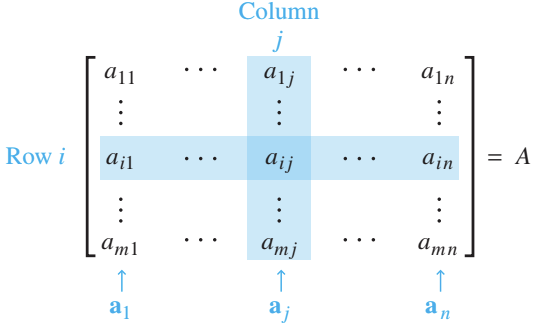
\includegraphics[width=0.3\textwidth]{image.png}}
  \caption{Notación Matricial}
\end{figure}

Las \textbf{entradas diagonlaes} en una matris $A$ son $a_11, a_22, a_33, \dotsb$ y forman la \textbf{diagonal principal} de $A$

\begin{tcolorbox}[colback=blue!10!white,colframe=blue!60!black,title=Matrices Especiales]
    Una matriz Diagonal es una matriz cuadrada de $n \times n$, cuyas entradas no diagonales son cero. Un ejemplo es la matriz identidad de $n \times n$, $I_n$. 

    Una matriz de $m \times n$ cuyas entradas son todas cero es una \textbf{matriz cero} o \textbf{matriz nula} y se escribe como 0.
\end{tcolorbox}
 
\section*{Suma y Múltiplos Escalares}

Se dice que dos matrices son \textbf{iguales} si tienen el mismo tamaño y si sus columnas correspondientes son iguales. Si $A$ y $B$ son matrices de $m \times n$, entonces la \textbf{suma} $A + B$ es la matriz de $m \times n$ cuyas columnas son las sumas de las columnas correspondientes en $A$ y $B$. \textbf{La suma $A + B$ solo está definida cuando $A$ y $B$ son del mismo tamaño.}

Si $r$ es un escalar y $A$ es una matriz, entonces el \textbf{múltiplo escalar} $rA$ es la matriz cuyas columnas son $r$ veces las columnas correspondientes de $A$. Al igual que sucede con los vectores, $-A$ significa $(-1)A$ y $A-B$ es igual que $A + (-1)B$

\begin{tcolorbox}[colback=green!20!white,colframe=green!80!black,title=Propiedades de una Matriz]
    Sean $A, B$ y $C$ matrices del mismo tamaño y sean $r$ y $s$ escalares.
    \begin{itemize}
        \item[i.] $A + B = B + A$ \hspace{80 mm} iv. $r(A + B) = rA + rB$ 
        \item[ii.] $(A + B) + C = A + (B + C)$ \hspace{60 mm} v. (r + s)A = rA + sA
        \item[iii.] $A + 0 = A$  \hspace{88 mm} vi. r(sA) = (rs)A
    \end{itemize}
\end{tcolorbox}

\section*{Multiplicación de Matrices}

Cuando una matriz $B$ multiplica a un vector \textbf{x}, trasnforma a \textbf{x} en el vector $B\mathbf{x}$. Si después ese vector se multiplica, a la vez, por una matriz $A$, el vector resultante es $A(B\mathbf{x})$

% Multiplicación de B y luego por A

Así, $A(B\mathbf{x})$ se produce a partir de \textbf{x} por una composición de mapeos. El objetivo es representar este mapeo compuesto como la multiplicación por una sola matriz, que se denota con $AB$, de manera que $$A(B\mathbf{x}) = (AB)\mathbf{x}$$

% Multiplicación por AB

Si $A$ es de $m \times n$, $B$ es de $n \times p$ y \textbf{x} está en $\mathbb{R}^p$, las columnas de $B$ se denotan como $\mathbf{b_j}, \dots, \mathbf{b_p}$ y las entradas de \textbf{x} como $ x_1,\dots, x_n$. Por consiguiente, $$B\mathbf{x} = x_1\mathbf{b_1} + \dotsb + x_p\mathbf{b_p}$$

Por la linealidad de la multiplicación $A$, 
\begin{equation*}
    \begin{aligned}
        A(B\mathbf{x}) &= A(x_1\mathbf{b_1} + \dotsb + x_p\mathbf{b_p})\\
                       &= x_1A\mathbf{b_1} + \dotsb + x_pA\mathbf{b_p}
    \end{aligned}
\end{equation*}

El vector $A(Bx)$ es una combinación lineal de los vectores $A\mathbf{b_1}, \dotsb, A\mathbf{b_p}$, usando las entradas de $\mathbf{x}$ como pesos. En notación matricial, esta combinación lineal se escribe como $$A(B\mathbf{x}) = \begin{bmatrix}
    A\mathbf{b_1} & A\mathbf{b_2} & \dotsb & A\mathbf{b_p}
\end{bmatrix}\mathbf{x}$$

\end{document}